Our focus in this Section will be put on continuously-monitored quantum systems. Opposite to the previously discussed single-shot scenarios, here we are interested in measuring the system repeatedly, which in the continuous limit leads to a \textit{measurement signal}. Here, we will give an introduction to the topic, and the interested reader is encouraged to complement our discussion with Refs.~\cite{wisemanbook,jacobs_2014,gardiner1985input, doherty1999feedback,wiseman1993interpretation}.

\begin{figure}[t!]
    \centering
    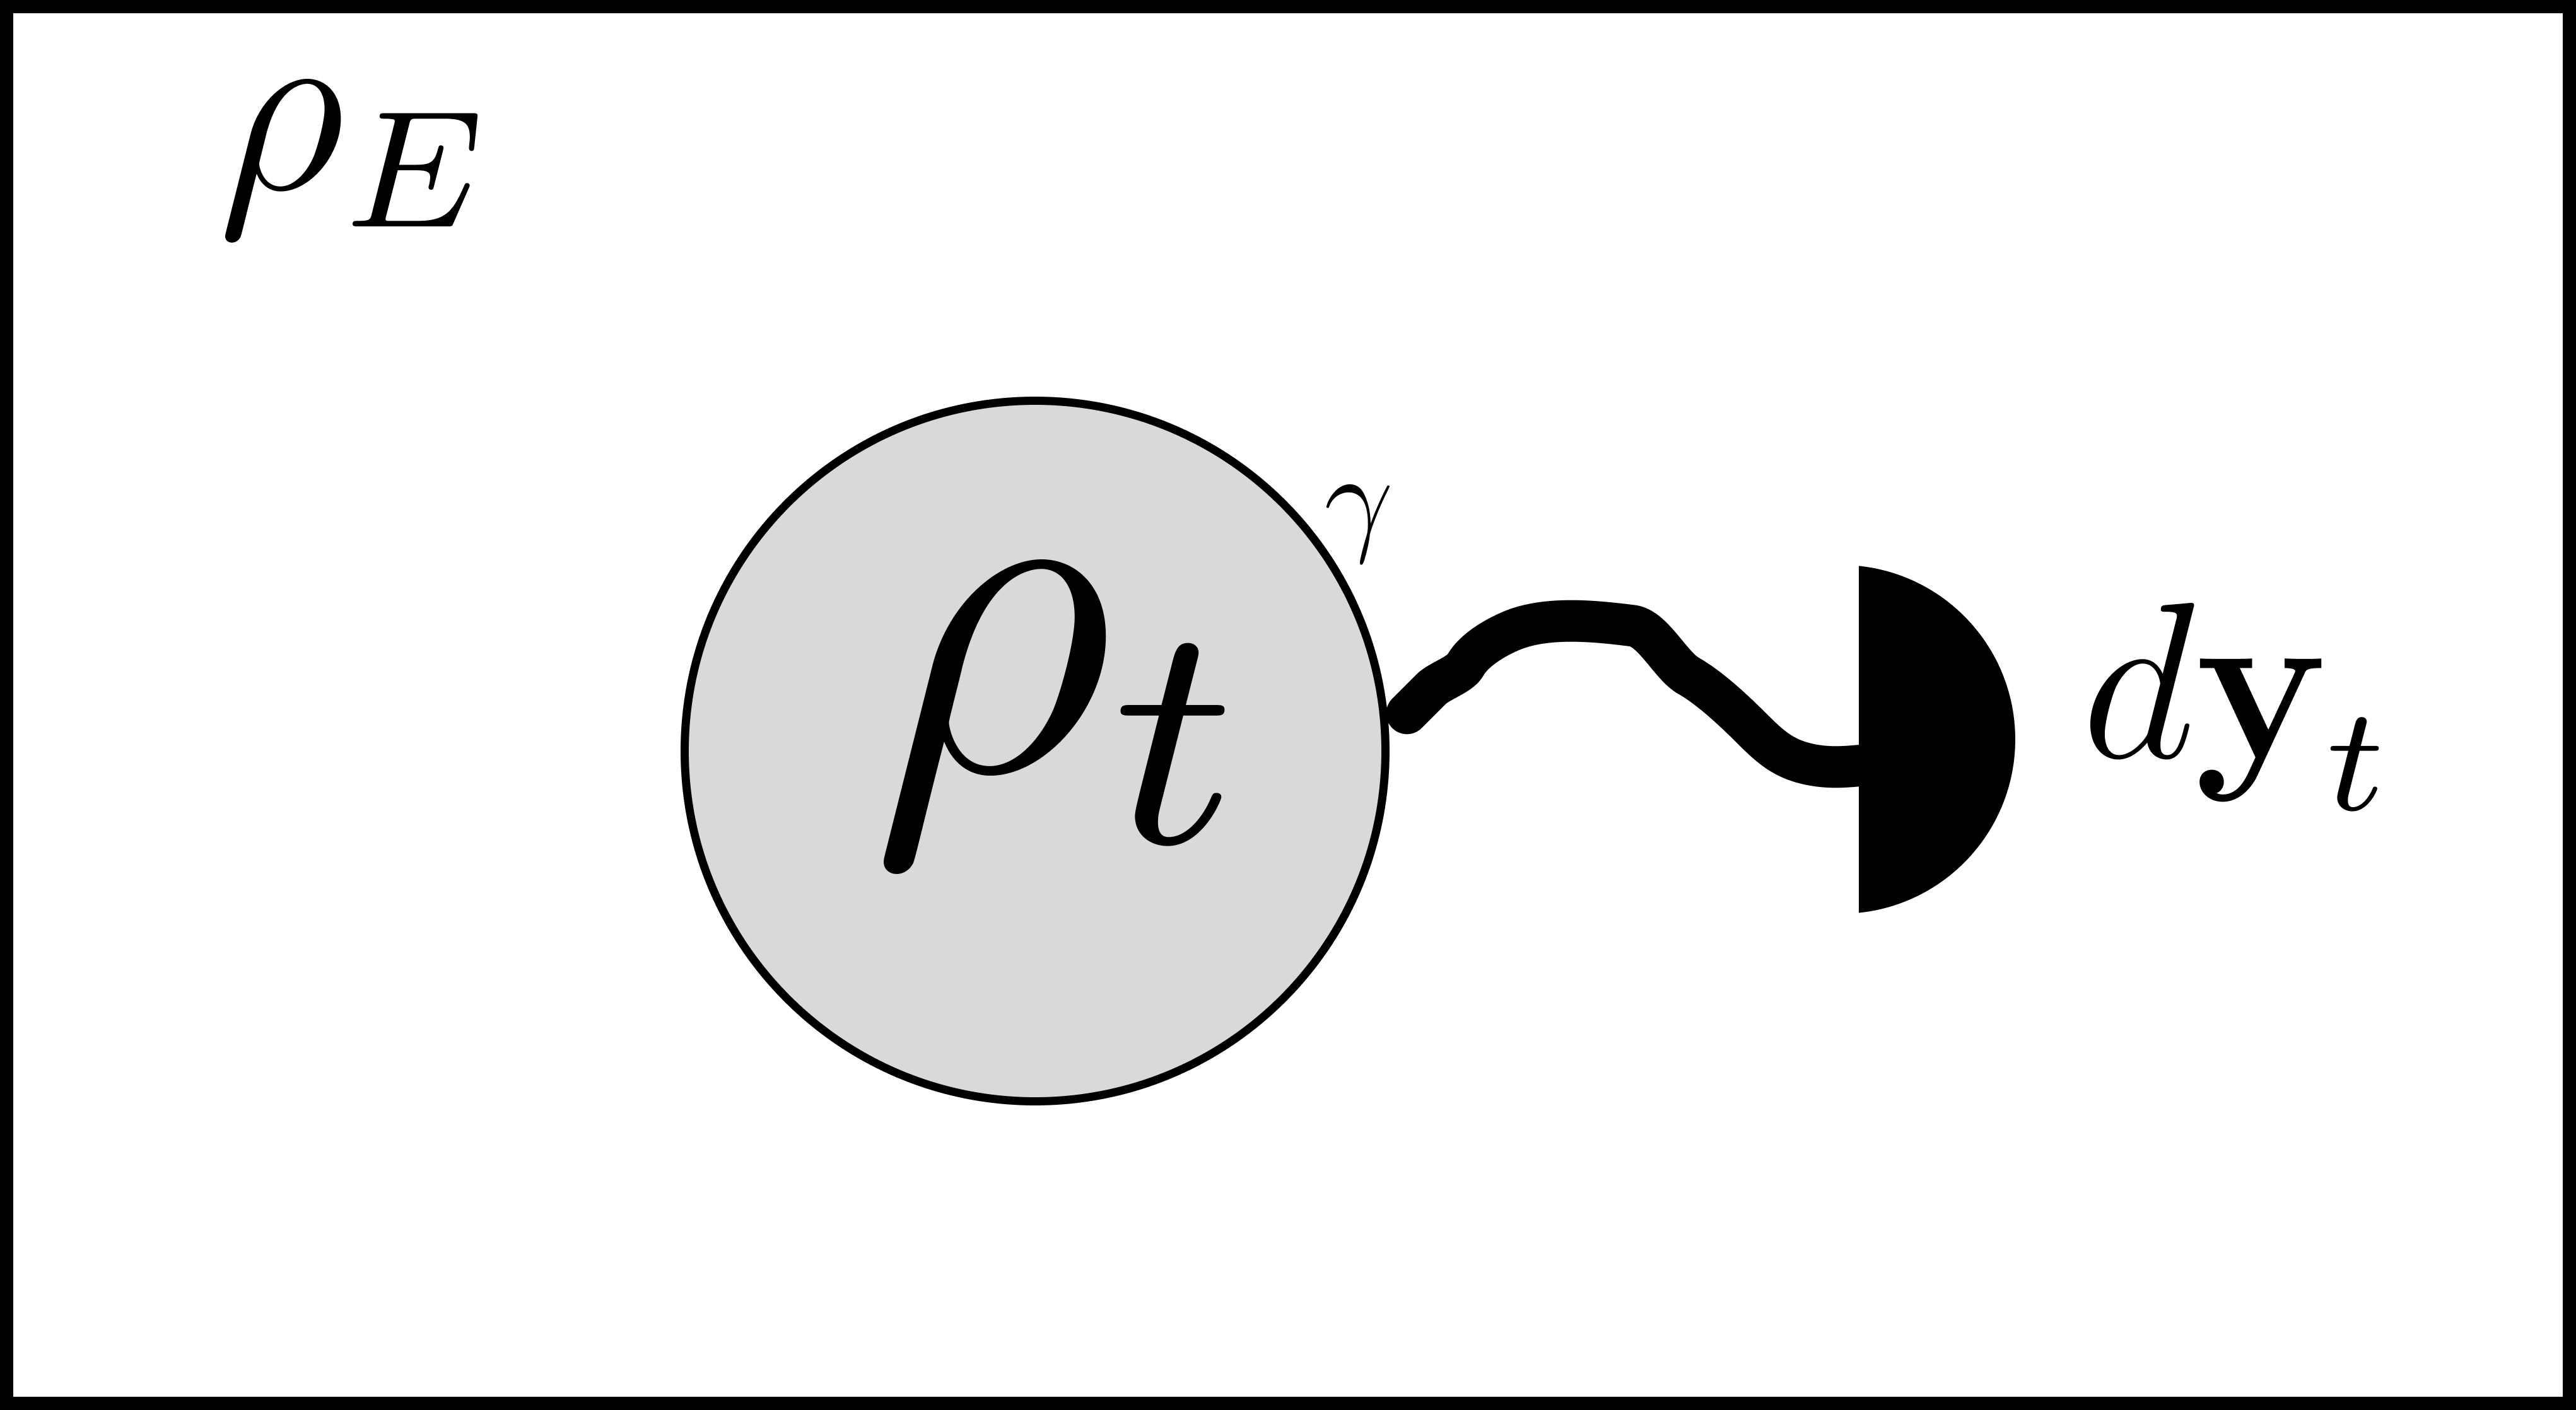
\includegraphics[width=1.\textwidth]{Figures/CMON/INTRO/cmon_esquema.png}
    \caption{We depict the continuously-monitored setting under consideration. This consists on an optomechanical cavity that stores a quantum system $\rho_t$, and whose decay rate is $\gamma$, and is coupled to a bosonic bath $\rho_E$, the latter being constantly measured. This gives rise to the measurement signal, whose (stochastic) value at time $t$ is denoted by $\dyt$.}
    \label{fig:cmon_scheme}
\end{figure}



\jccc{A quantum system is continuously-monitored by coupling an ancillary electromagnetic mode to it, and measuring such mode as}{The most direct  way to implement a continuous measurement on a quantum system is to  couple it an electromagnetic auxiliary mode that is subsequently measured via photon-counting or dyning measurements as,} shown in Fig.~\ref{fig:cmon_scheme}. While several physical scenarios allow for this kind of detection --- among them atomic sensors~\cite{Jimenez2018signal} and mesoscopic electrometers using quantum dots~\cite{Lu2003}---, we will focus on optomechanical cavities~\cite{Aspelmayer2014cavity} \jccc{which are able to \textit{store} the quantum system that we want to monitor.}{.}.

To this end, we begin in Sec.~\ref{ssec:1_cmon_physics} by providing some insight on optical cavities and their interplay with measurements done \jccc{on the bosonic bath.In particular, we are interested in how such a measurement affects the evolution of the system stored in the cavity, whose overall dynamics is formally described by an \textit{stochastic master equation} (SME)}{ on the the light that leaks out of the cavity. Since such measurement outcomes are stochastic the evolution of the system will be given by a stochastic master equation (SME).}\jccc{  Thus, in}{In} Sec.~\ref{ssec:contphoto} we derive an SME for the case of a single optical mode stored in the cavity and photon-detection done on the outside modes \jcc{, leading to a SME driven by point process (measurement record is a a sequence of photon clicks).} We then consider homodyne detection in Sec.~\ref{ssec:1_cmon_homodyne}, where the measurement signal becomes continuous, and a Wiener noise appears in the play. Next, a general equation for a continuously-monitored Gaussian system is discussed in Sec.~\ref{ssec:1_cmon_gaussian}.
Finally, in Sec.~\ref{ssec:1_cmon_model} we introduce the optomechanical model that we consider in Chapter~\ref{chapter:CMON}; \jccc{such}{which} is used as a testbed for our approaches to the statistical inference problems considered in that Chapter.

\subsection{Cavity emission and photon-detection}\label{ssec:1_cmon_physics}
Optical cavities consist on convex mirrors faced \jccc{toghether}{together} at some \jccc{(possibly varying)}{} distance, \jcc{where light can be stored in a standing wave mode for long periods of times.  In order to access the cavity mode one the mirrors can be made  be  slightly transmissive, as in Fig.~\ref{fig:cavityCMON}. This allows to retrieve information by measuring the leaked photons and to pump the cavity field by an external laser. Since light is trapped inside the cavity for long periods of times, placing a quantum system inside it,  is one of the most effective means of coupling quantum systems to light.

The leaked light occupies travelling modes (free propagating), which means  such photons will never interact again with the system. This allows one to describe the evolution of the cavity mode, as a markovian dynamics corresponding to a electromagnetic (bosonic) cavity mode coupled to a bosonic bath consisting of the free-propagating modes ---for optical modes, this bath is taken to be at zero temperature, i.e. the vaccuum state, but  the formalism also allows to consider non-zero temperatures, that are present for example in the baths of optomechanical systems. }



\jccc{
where a quantum system (\textit{e.g.} light and/or a mechanical system such as an atom) is stored. Since mirrors are not perfect, some of the light stored in the cavity leaks, and by measuring the leakage we can effectively measure the system inside the cavity. In practice, one of the mirrors has a transmission rate much smaller than the other, and thus we do only consider a single leakage, as depicted in Fig.~\ref{fig:cavityCMON}.}{}

\begin{figure}[t]
    \centering
    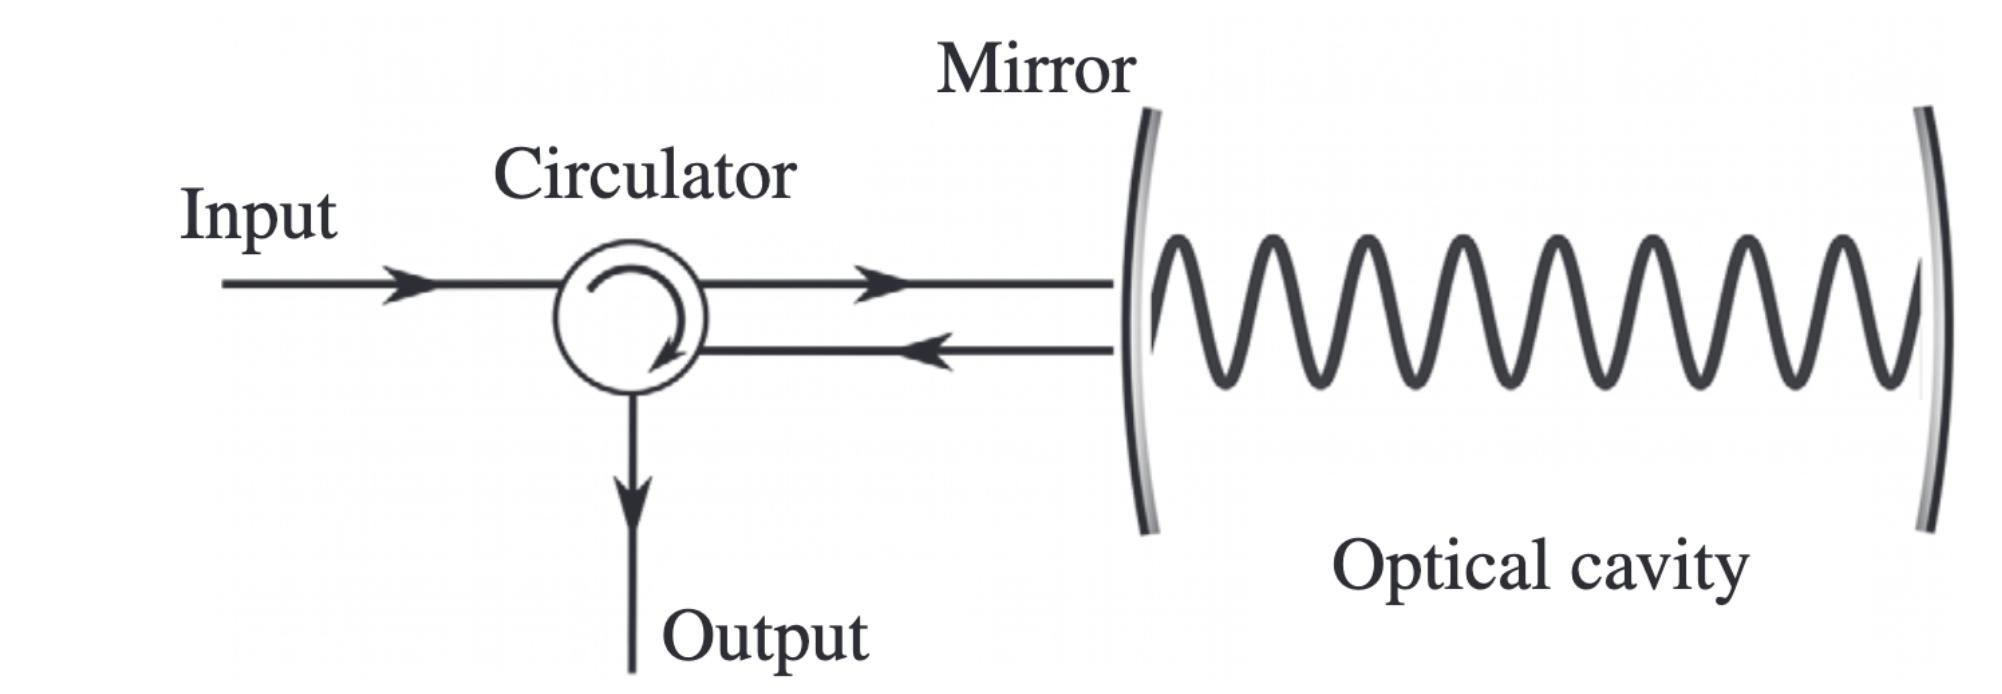
\includegraphics[width=1.\textwidth]{Figures/CMON/INTRO/cavitiy_jacobs.png}
    \caption{An optical cavity is depicted (image taken from Ref.~\cite{jacobs_2014}, Ch.3). Here, light is input (and output) to (and from) the cavity by the same mirror, and such two modes are splitted by the circulator.}
    \label{fig:cavityCMON}
\end{figure}

\jccc{The cavity is in contact with a bosonic bath, which consists of electromagnetic modes.}{}We denote the cavity's decay rate by $\gamma$ \jcc{(depending on the transmissivity of the mirror),  the annihilation operator for the cavity mode  $a$ and the anhilliation operator at detection time $t$ , $b_t$.} By approximating the bath's autocorrelation function as a delta-function, which makes the bath Markovian\footnote{This matter is discussed further in Sec.3.3. and Sec.3.11 of Ref.~\cite{wisemanbook}} we obtain the following commutation for the bosonic bath's operators in the interaction picture w.r.t. system's Hamiltonian:%~\cite{wisemanbook,wiseman1993interpretation,gardiner1985input}
\eq{commbathdelta}{\comm{b_t}{b_{t'}^\dagger} = \delta(t-t').}
Under the rotating-wave approximation, the interaction potential between cavity and bath is modelled to be
\eq{eee}{V_{IF} = -\ii \sqrt{\gamma}\big( b_t a^\dagger - b_t^\dagger a \big),}
and describes the exchange of excitations between each other. However, due to the singularity appearing in Eq.~\ref{eq:commbathdelta}, we must be careful when studying the dynamics generated by $V_{IF}$. A convinient approach is that of treating $b_t$ \textit{a la Ito}~\cite{wiseman1993interpretation}\footnote{Ito calculus is one of the most widely used theories for stochastic calculus, which allows to compactly write and solve differential equations for stochastic variables in a similar was as for standard differential equations for deterministic continuos functions. While working with Ito calculus, one proceeds similarly than traditional calculus but taking into account a few important rules. We briefly discuss this topic in Sec.~\ref{ssec:ito}.}. Thus, an infinitesimal operator is defined as
\eq{infidB}{dB_t = b_t dt,} with commutation relations:
\equ{\comm{dB_t}{dB_t^\dagger} = dt,} which shows that the operator $dB_t$ can be understood as being order $\sqrt{dt}$. With the re-defined bath's operators, we can now study how an infinitesimal evolution looks like. Here, we must be careful when performing expansions, since the $\sqrt{dt}$ scaling requires to go up to second order terms. To do this, we consider the infinitesimal evolution generated by $V_{IF}$ in Eq.~\ref{eq:eee}, and we get
\begin{align}
U(t+dt,t) &= e^{\sqrt{\gamma}(a \; dB_t^\dagger - a^\dagger dB_t)} \nonumber\\
&= \mathbb{I} + \sqrt{\gamma} \big( a  \; dB^\dagger - a^\dagger dB\big) - \frac{1}{2} \gamma a^\dagger a \;dt - \frac{\gamma}{2}\llaves{a^\dagger, a} dB^\dagger dB  \\ & \spacee+\frac{\gamma}{2} \big(a^2 {dB^\dagger}^2 + {a^\dagger}^2 dB^2\big) \nonumber,
\end{align}
which describes an infinitesimal evolution of the joint system, in the interaction picture.

We will now assume that the bosonic bath is always found in the ground-state $\ket{0}$, and that at each time-step $t$, the system interacts with a new copy of such ground-state \jcc{(i.e., with a new mode $b_{t}$)}. Let us also assume that system's state is given by $\ket{\psi(t)}$. With this, the global state at time $t+dt$ is given by
\equ{U(t+dt,t)\ket{0}\ket{\psi(t)} = \Big(\mathbb{I} - \frac{\gamma}{2}a^\dagger a dt\Big)\ket{0}\ket{\psi(t)} + \gamma dB^\dagger \ket{0} a \ket{\psi(t)}.}
Under these assumptions, the probability of finding an excitation in the bath is given by
\equ{p_1(dt) = \gamma \langle 0 | dB dB^\dagger |0\rangle \bra{\psi(t)} a^\dagger a \ket{\psi(t)},} which turns out to be small if we recall that $dB dB^\dagger = dt$.\footnote{This relationship holds since we only keep the non-normally ordered operators in bath's commutation relations, as such is assumed to be in the ground-state}

\jcc{}

\jccc{Up to now, we have discussed a model on how information can be extracted out of a cavity, by measuring the bath. Here, excitations of the bath are linked to the mean photon number inside the cavity, and thus we can readily acquire information about the latter by repeatedly measuring the former. We will now formalize this by study the evolution of the quantum system stored in the cavity when we repeatedly perform these kind of measurements.}

\subsection{Continuous photon-detection}\label{ssec:contphoto}



\jcc{To begin our study of conditional post-measurement states, we will consider the photon-detection example outlined in the previous section, but we will also include the action of the system's hamiltonian. By
direct identification of the post-measurement  (unnormalized) conditional states are given by
$\ket{\psi_0(t+dt)} =M_{0}\ket{\psi(t)}$ and $\ket{\psi_1(t+dt)} =M_{1}\ket{\psi(t)}$  where the two
 Krauss operators are:}
\begin{align}\label{eq:photocoM}
M_0 &= \mathbb{I} - \Big(\frac{R}{2} + \ii H \Big) dt\\
M_1 &= c \sqrt{dt},
\end{align}
where $H$ stands for the system's Hamiltonian\footnote{We will drop the hat notation for operators in this Section.}, $dt$ is an infinitesimal amount of time,  \jccc{$c$ can be linked to cavity's anhilation operator introucef in the previous Section as per}{ $c = \sqrt{\gamma}a$, with $\gamma$ being the cavity's decay rate and  $R=c^\dagger c$}.

By dropping terms of $\mathcal{O}(dt^2)$, it is straightforward to check that $\llaves{M_0, M_1}$ constitute a valid quantum instrument ($M_{0}^{\dagger} M_{0}+M_{1}^{\dagger} M_{1}=\mathbb{I}$), and that the unconditional post-measurement state, \textit{e.g.} the state of the system at time $t+dt$ when not recording the measurement outcome, recovers the Libland form in Eq.~\ref{eq:libland} for the cavity emission model:
\begin{align}\label{eq:cavityemission}
\rho(t+dt) &= M_0 \rho\jcc{(t)} M_0^\dagger + M_1 \rho(t) M_1^\dagger \\
&= \rho(t) - \ii \left[ H,\rho(t) \right] dt + c^\dagger \rho c - \frac{1}{2}\llaves{c^\dagger c, \rho(t)}=:\rho(t)+d\rho(t)
\end{align}

\jcc{
}.


\jcc{}.


  \jccc{be dropped}{left implicit} from now on.

\jcc{} \jccc{the we can deduce an equation for the density matrix of the system, by studying the evolution of the projector $\proj{\psi(t)}$, which after some trivial simplifications reads}{}






\jcc{

}



\subsection{Continuous homodyne detection}\label{ssec:1_cmon_homodyne}
We have previously study a stochastic master equation for an specific \textit{unraveling} of unconditional dynamics, namely photon-detection. In such case, a detection induces a \textit{quantum jump} on the system's density matrix, with a probability that is proportional to $dt$, as given by Eq.~\ref{eq:pointpro}. Here, we will study a different unraveling of the dynamics.

The existence of different unravelings arises from the invariance of the master equation --- \textit{i.e.} the undonditional open quantum system dynamics revisted in Sec.~\ref{ssec:1_intro_open} --- under certain transformations (see also Eq.~\ref{eq:invalibland}) of the form
\begin{align}
c &\rightarrow c + \alpha \\
H &\rightarrow H - \frac{\ii}{2}\big(\bar{\alpha}c - \alpha c^\dagger),
\end{align}
with $\alpha \in \mathbb{C}$. This is equivalent to a different (unitarily equivalent) Kraus representation:
\begin{align}\label{eq:homPOM}
M_0 &\rightarrow\tilde{M}_0(t) = \mathbb{I} - dt\big(\ii H + \frac{\bar{\alpha}c - \alpha c^\dagger - (c+\alpha)^\dagger(c+\alpha)}{2}) \\
M_1  &\rightarrow \tilde{M}_1(t) = \sqrt{dt}(c+\alpha).
\end{align}
This transformation can physically be achieved by mixing the input field with a strong local oscillator (L.O.) by a low transmissivity beam-splitter (BS)\footnote{To see this, let the transmissivity of the BS be $\eta\sim1$, and let the intensity of the L.O. be $\frac{\alpha}{\sqrt{1-\eta}}$; the reflected mode will then be \equ{\sqrt{\eta} c + \alpha,}assuming we treat the local oscillator classically, an approximation valid when the intensity of the L.O. is sufficiently high~\cite{serafiniBOOK}. From here, since $\sqrt{\eta}\sim1$, we get the desired transformation.}, as shown in Fig.~\ref{fig:direhom}, which corresponds to direct homodyne detection. In turn, let us restrict to $\alpha\in\mathbb{R}$, then a detection (as defined in the previous section) happens with probability
\begin{align}
p_1(dt) = \mathbb{E}\corch{dN} &= \tr{\rho (c+\alpha)^\dagger(c+\alpha)} dt \\
&= \tr{\rho \big(c^\dagger c + \alpha (c+c^\dagger) + \alpha^2\big)}\\
&= \tr{\rho \big(c^\dagger c +  \alpha q + \alpha^2\big)},
\end{align}
where $q = c+c^\dagger$ stands for the position quadrature\footnote{We will momentaneously drop the $\sqrt{2}$ factor to ease the notation}. Thus, if $\alpha\gg\expect{c^\dagger c}$, photon-detection at the reflected port is equivalent (up to a constant) to measuring the $q$ quadrature. This is corresponds to the case of direct \textit{homodyne} detection, which was introduced in Sec.~\ref{ssec:1_cv_measurements}; we will here consider the direct homodyne detection, which is realized by mixing the system with a strong local oscillator by a low transmissivity beam-splitter, as shown in Fig.~\ref{fig:direhom}.

\begin{figure}[t!]
    \centering
    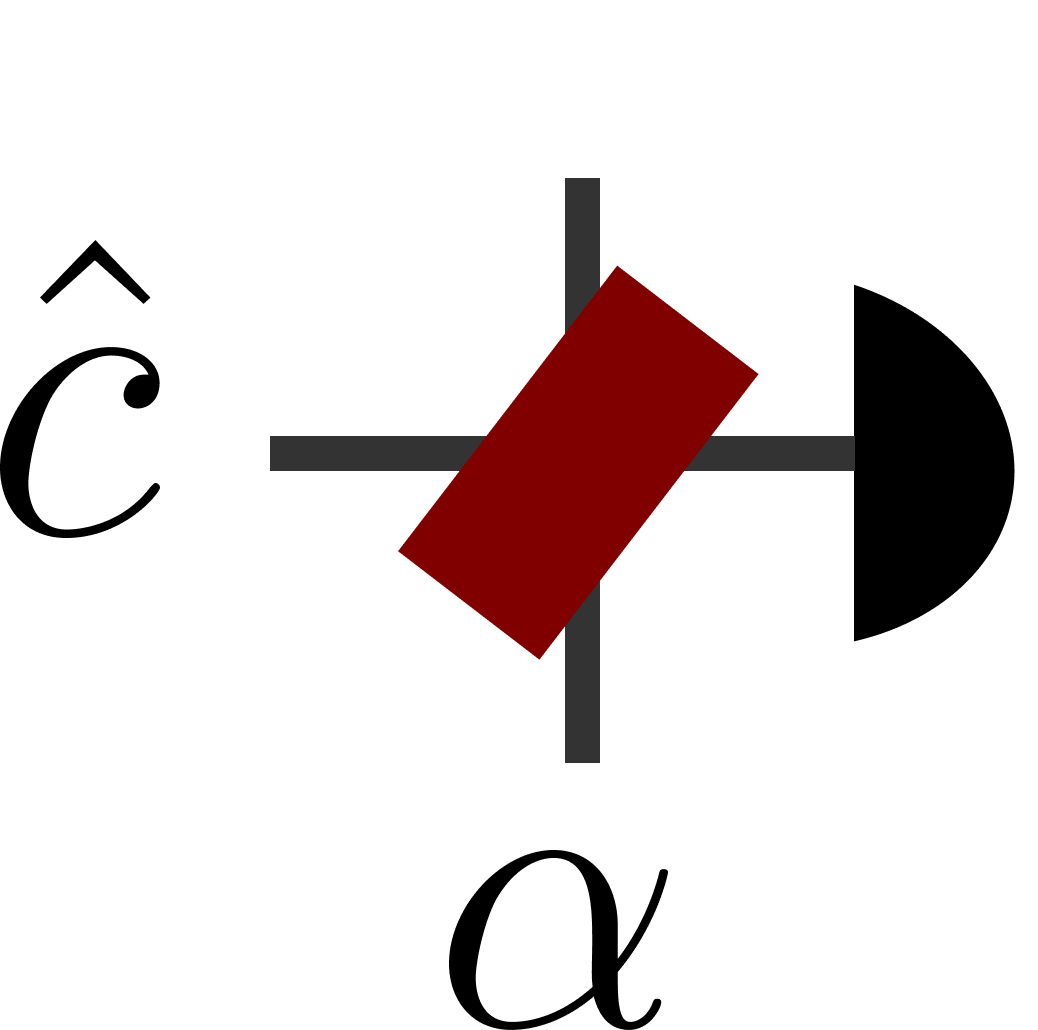
\includegraphics[width=0.25\textwidth]{Figures/CMON/INTRO/homodyne.png}
    \caption{We sketch a direct homodyne detection. The beam-splitter is chosen such that the reflected part (which is subsequently measured) has only a small contribution of the local oscillator, and is dominated by the original signal associated to the system we are measuring.}
    \label{fig:direhom}
\end{figure}

Repeating the same procedure outlined by the end Sec.~\ref{ssec:contphoto}, but now with the transformed POVM $\tilde{\mathcal{M}} = \llaves{\tilde{M}_0(t), \tilde{M}_1(t)}$, we get a stochastic master equation that reads
\begin{align}
d\rho = \mathcal{G}[c+\alpha] \rho dN + dt \mathcal{H}\Big[\ii H + \alpha c + \frac{c^\dagger c}{2}\Big].
\end{align}
From here, we are aim to take the continuous limit, in which the photocurrent is approximated by a continuous function of time. This corresponds to the ideal limit of homodyne detection, in which the intensity of the local oscillator goes to infinity. In particular, we are interested in a regime under which the number of detections per time is high and changes in the system are small. In such regime, we obtain a \textit{Belavkin-Zakai} equation, which is yet another quantum stochastic master equation, that describes the continuous homodyne-monitoring of a quantum system. We will now derive such equation by making expansions in terms of the local oscillator intensity, following Ref.~\cite{wisemanbook}\footnote{Note that there are alternative ways to derive this equation. For instance by straightfowardly considering the action of a Gaussian measurement on the quantum state and Taylor-expanding it in terms of $dt$~\cite{jacobs_2014, JacobsStraightfoward2006}, or considering the interaction between a Gaussian system, bath and measurement\cite{serafini2017quantum,Genoni2016conditional}, although this formalism is focused on Gaussian systems, and directly leads to the set of stochastic linear equations for mean and covariance of the quantum state, which we discuss later on, bypassing stochastic master equations.}.

We begin by considering a small time-interval $\delta t = \mathcal{O}(\alpha^{-\frac{3}{2}})\ll1$\footnote{The only purpose of considering $\delta$ rather than $d$ is that we take a limit in terms of local oscillator intensity by the end of this discussion}, that results in an expected number of detections,
\eq{edng}{\mathbb{E}[\delta N] = \delta t\;\tr{\rho (\alpha^2 + \alpha q + c^\dagger c)} = \mathcal{O}(\alpha^{\frac{1}{2}}),}
which is large in comparison to system's evolution (since $\delta t = \mathcal{O}(\alpha^{-\frac{3}{2}})$). Under this choice of scaling, the detection probability is algo large $p_1(\delta t) = \mathcal{O}(\sqrt{\alpha})$.

As pointed out in Sec.~\ref{ssec:1_cv_measurements}, $\delta N$ is a Poissonian random variable. However, it is possible --- since the number of detections happening per $\delta t$ is large --- to approximate such probability distribution by a normal distribution~\cite{wisemanbook,wiseman1993quantum} (intuitively we can understand this as a central-limit theorem) with a mean-value given by Eq.~\ref{eq:edng} and variance
\eq{variaCMON}{\sigma^2= \delta t \big(\alpha^2 + \mathcal{O}(\alpha^{\frac{3}{2}})\big).}
By recurring to Ito calculus, Eq.~\eqref{eq:variaCMON} can be written compactly as
\eq{dnito}{\delta N = \alpha^2 (\delta t) \corch{1 + \frac{\expect{q}(t)}{\alpha}    } + \alpha \delta W,}
where $\delta W$ describes a differential white noise, \textit{e.g.} a zero-mean normal random variable whose variance is $\mathbb{E}[\delta W^2] = \delta t $.

It is now time to make a brief pause, and jump to revise Ito calculus. The interested reader is referred to Ref.~\cite{gardiner2004handbook}, where further details about this topic can be found.

\subsection{Intermezzo II: Ito calculus}\label{ssec:ito}

\jcc{}

\jccc{ While the differential noises $dW$ are of stochastic nature, in Ito calculus their square is a deterministic quantity, \textit{e.g.} $dW^2=dt$, and thus we deem them order $\sqrt{dt}$, hence $dW dt = 0$}.




····


Recalling that the evolution of cavity's system under the transformed measurement operators of Eq.~\eqref{eq:homPOM} reads
\equ{\delta \rho = \delta N(t)\mathcal{G}\Big[c+\alpha\Big]\rho - \delta t \mathcal{H}\Big[\ii H + \alpha c + \frac{c^\dagger c}{2}\Big]\rho,}
we can now work the $\mathcal{G}[c+\alpha]$ term and expand it in powers of $\alpha^{-1}$; this means keeping the terms up to $\frac{1}{\alpha^2}$ arising by Taylor expanding up to the second order the normalization in $\mathcal{G}$ (see Eq.~\ref{eq:superGH}). After such expansion, we obtain
\begin{equation}\label{eq:ddynexp}
\delta \rho = \delta N(t) \Big[ \frac{\mathcal{H}[c]}{\alpha} + \frac{\mathcal{G}[c] - \expect{q} \mathcal{H}[c]}{\expect{c^\dagger c}} \Big] \rho - \delta t \mathcal{H}\Big[\ii H + \alpha c + \frac{c^\dagger c}{2}\Big]\rho
\end{equation}
Now, plugging the Ito form of $\delta N$ into Eq.~\ref{eq:ddynexp}, we get
\begin{equation*}
\delta \rho = \Big( \alpha^2 \delta t \Big[ 1 + \frac{\expect{q}}{\alpha}\Big] + \alpha \delta W \Big) \Big( \frac{\mathcal{H}[c]}{\alpha} + \frac{\mathcal{G}[c]\expect{c^\dagger c} - \expect{q}}{\alpha^2} \Big)
\rho + \delta t \mathcal{H}\Big[-\ii H - \alpha c - \frac{c^\dagger c}{2}\Big]\rho.
\end{equation*}
From here, we can expand all the products on the above equation and keep terms of order $\frac{1}{\sqrt{\alpha}}$ or higher. Finally, taking the limit $\alpha\rightarrow \infty$ we get the desired Belavkin-Zakai equation for homodyne measurement:
\begin{align}\label{eq:1introBELAVKIN}
d\rho &= dt\Big(- \ii \Comm{H}{\rho} + \mathcal{D}[c]\rho\Big) + \mathcal{H}[c]\rho \;dW\\
\mathcal{D}[c]\rho &:= c\rho c^\dagger - \llaves{\frac{c^\dagger c}{2},\rho} \\ \nonumber
\mathcal{H}[c]\rho &= c\rho + \rho c^\dagger - \tr{(c+c^\dagger)\rho},\nonumber
\end{align}
\jccc{where to facilitate reading we included the definitions of the super-operatos $\mathcal{D}[c]$ and $\mathcal{H}[c]$ introduced before.}{[D no lo habias introducdio aun,no?]}

The last equation describes the evolution of a Markovian system which is subject to a continuous monitoring under homodyne detection. Similar to photon-detection situation, when averaging out over possible measurement outcomes, the Libland form is recovered.% (\textit{i.e.} the non-selective master equation).

On the other hand, a measurement \textit{signal} arises, which is also a continuous function of time. To see this, let us return to the Ito expression for $\delta N(t)$, namely
\equ{\delta N(t) = \alpha^2 \delta t \left[ 1 + \frac{\expect{q}(t)}{\alpha}\right] + \alpha \; \delta W,}
which after subtracting the intensity of the local oscillator we get
\begin{equation}
dy(t) = \underset{\alpha \rightarrow \infty}{\text{lim}} \frac{\delta N (t) - \alpha^2\delta t}{\alpha} = \expect{q}dt + dW,
\end{equation}
where clearly $\expect{q}$ is time-dependent and also the Wiener noise. \jcc{}
%\jccc{Of course, by averaging over all possible measurement record
% by choosing the right cross graining time interval (long enough to average the effect of several detection clicks, but short enough compared to the dynamics of the system), the non-continuous quantum jump evolution described by Eq.~\ref{eq:foto} by a continuous, diffusive evolution, that corresponds to monitor the $q$ quadrature of the system. We will now comment on how imperfect detection is modelled.}{}

\subsection{Imperfect detection}
First, the case of inefficient detection, in which the efficiency of the photodetector $\eta$ is less than unity. In this case, the master equation describing cavity emission of Eq.~\ref{eq:cavityemission} can be understood as
\begin{align}
d\rho = -\ii \Comm{H}{\rho}dt + (1-\eta)\mathcal{D}[c] \rho dt + \eta \mathcal{D}[ c]\rho,
\end{align}
and only unravel the last term\footnote{note that $\mathcal{D}[\sqrt{\eta} c] = \eta \mathcal{D}[c]$.}, resulting in a modified stochastic master equation that for the homodyne case Eq.~\ref{eq:1introBELAVKIN} is slightly modified to read
\begin{align}\label{eq:inefficientDETECTION}
d\rho = -\ii\comm{H}{\rho}dt + \mathcal{D}[c] \rho dt + \sqrt{\eta} \mathcal{H}[c] \rho \;dW.
\end{align}
Moreover, the homodyne measurement signal for the inefficient detection case reads
\begin{align}\label{eq:1_cmon_ineff_measu}
dy = \sqrt{\eta} \langle q \rangle dt + dW.
\end{align}

The remaining refinement that we consider deals with the bosonic bath, which so far has been assumed to be in the ground-state. However, we might assume that the cavity is in contact with a thermal bath. Deriving stochastic master equations when measuring such thermal bath turns to be an obscure subject~\cite{wisemanbook,jacobs_2014}. However, we can assume that the thermal bath is just an extra reservoir which we do not measure. In this case, we recall that the master equation (for the cavity plus thermal bath only) reads:
\begin{align}\label{eq:master_thermal}
\frac{d\rho}{dt} = -\ii\Comm{H + \ii(\bar{\beta} c + \beta c^\dagger)}{\rho}\jcc{(}n_{th}+1) + \mathcal{D}[c] \rho + n_{th} \mathcal{D}[c^\dagger] \rho,
\end{align}
where $n_{th}$ is the average number of photons in the cavity and depends on bath's temperature, and we observe that the mean value of the incoming field, $\beta dt = \expect{dB}$, has a driving effect on the cavity\cite{wisemanbook}. This driving term induces a constant shift in cavity's quadratures that in the following will be dismissed.

As stressed in Sec.~\ref{sec:1_cv}, measuring system's quadrature belongs to the set of Gaussian measurements, and as such preserves the gaussian character of (an initially gaussian) state. This motivates the following Section, in which we study the quadratures dynamics of a quantum system under continuous homodyne detection.

\subsection{The Gaussian case}\label{ssec:1_cmon_gaussian}
In the previous Sections we have studied the dynamics of a cavity when its bath is being continuously-monitored, and also discussed a model for imperfect detections. We will now discuss the dynamics structure when the system is assumed Gaussian. We have introduced Gaussian systems in Sec.~\ref{ssec:intro_cv_gaussianinfo}, and also studied how a Gaussian map modifies the first moments of a Gaussian state in Sec.~\ref{ssec:1_cv_channels}. Opposite to such Section, we are here interested in studying the \textit{conditional} diffusive dynamics of the Gaussian system, arising as a consequence of continuously-monitoring the bath coupled to it.

Our discussion follows \textit{the Wiseman approach}~\cite{wisemanbook,Wiseman2005optimal,wiseman1993interpretation}, which consists on deriving dynamical equations for the moments of a Gaussian state \textit{from} the stochastic master equation of Eq.~\ref{eq:1introBELAVKIN}. However, we remark that for the Gaussian case, the same equations can be derived by straightfowardly working with the moments, and assuming an specific (Gaussian) structure for the interaction between bath's and system's modes. This constitutes the \textit{Serafini approach} one, and while it will not be discussed here, the interested reeader can consult Refs.~\cite{serafiniBOOK,Genoni2016conditional}.

For the sake of simplicity, we will restrict to a single-mode quantum system. We consider an equation of the form in Eq.~\ref{eq:1introBELAVKIN}:\footnote{Let us remark that while we derived such equation for an optical cavity, it can be used to describe more complex systems, such as quantum dots coupled to nano-mechanical resonators~\cite{wisemanbook}. Morever, by the end of this Section we will consider a slightly more complex model for the cavity, and discuss an scenario where a mechanical mode is also considered.}
\begin{align}\label{eq:cmon_optimal1}
d\rho &= \mathcal{L}_0 \rho dt + \mathcal{H}[c]\rho \; dW_t,
\end{align}
where $c$ is an arbitrary system operator ($c=\sqrt{\gamma}a$ in the cavity model), and $\mathcal{L}_0$ is the Liblandian describing the non-diffusive open-quantum dynamics (that takes into account interaction with additional modes).

We recall that Gaussian states are generated by Hamiltonians which are at most quadratic in system's quadratures:
\begin{align}
H = \frac{1}{2} \rop G \rop - \rop^T \Omega B \textit{u}(t),
\end{align}
where $G$ is the Hamiltonian matrix (\textit{i.e.} $G$ is real and symmetric)\footnote{Note our change in notation with respect to Sec.~\ref{sec:1_cv}, \textit{e.g.} $G\equiv H$ in Eq.~\ref{eq:hamiGauss}.} and included a possible time-dependent drive $\textit{u}(t)$ that enters in the Hamiltonian as a linear term (\textit{e.g.} a displacement due by a driving force). Also, we recall that $\Omega$ is the symplectic form defined in Eq.~\ref{eq:cv_ccr}, and that system's mean and covariance are defined as $\rbar = \expect{\rop} = \tr{\rho \rop}$ and $\cov_{nm} = \expect{\Delta \rop_n \Delta \rop_m} + \expect{\Delta \rop_m \Delta \rop_n}$, with $\Delta \rop_i = \rop_i - \expect{\rop_i}$, and $\rop = (q, p)$.
Moreover, the transformation $\tilde{C}$ mapping system's quadratures with the operator $c$ in Eq.~\eqref{eq:cmon_optimal1} is defined via $c = \tilde{C} \rop$, which for the cavity model reads $\tilde{C}=\sqrt{\gamma}\Big(1, \ii\Big)$.

If we only consider the unconditional dynamics, given by the Liblandian $\mathcal{L}_0$, and use the canonical commutation relations in Eq.~\ref{eq:cv_ccr}, we can derive a dynamical equation for the first two moments $\rbar, \cov$:
\begin{align}\label{eq:cmon_unco}
d \rbar &= \Big(A\rbar  + B\textit{u}(t)\Big) dt\\
d \cov &= \Big(A \cov + \cov A^T + D \Big) dt, \nonumber
\end{align}
where $A = \Omega( G + \text{Im}[\mathcal{C}])$ and $D = \Omega \text{Re}[\mathcal{C}]\Omega^T$ and $\mathcal{C} = \tilde{C}^\dagger \tilde{C}$~\cite{Wiseman2005optimal}. We note that Eq.~\ref{eq:cmon_unco} is just a different parametrization of the Gaussian evolution described in Eq.~\ref{eq:1_cv_gaussianCPmap}.
However, if we now consider the \textit{conditional evolution}, that arises from continuously-monitoring via homodyne detection and is captured by Eq.~\ref{eq:cmon_optimal1}, a stochastic term is expected to appears in moments' dynamics.

To this end, let us re-write the measurement signal in Eq.~\ref{eq:1_cmon_ineff_measu} in terms of system's quadratures\footnote{We will now recover the factor 2 dropped when defining $q = a + a^\dagger$ in the previous Section} as
\eq{signal_dy}{\dyt = C( \rbar dt +  C^{-1})\dwt,}
with $C = \sqrt{4 \eta \gamma}\Big(\begin{matrix}1&0\\0&0\end{matrix}\Big)$. Here, our notation $\dyt$ accounts for the fact that two components are in principle obtained when monitoring the first moment of the quantum state. For homodyne detection this implies that the second component is uninformative and always zero-valued, a fact also stressed by including the pseudo-inverse of $C$ in the above equation.

Computing the first moments --- \textit{e.g.} by taking the corresponding expectation values in Eq.~\ref{eq:cmon_optimal1}, where we take into account the interaction with a thermal math in $\mathcal{L}_0)$ ---, and using Isserlis' theorem to simplify the covariance evolution~\cite{JacobsStraightfoward2006}, we get the following system of lineal stochastic equations:
\begin{align}\label{eq:cmon_LINEALSYSTEM}
d\rbar_t &= \big(A - \chi(\cov_t) C\big) \rbar_t dt + \chi(\cov_t) \dyt = A \rbar_t dt + \chi(\cov_t) dW_t \\
d\cov_t &= A \cov_t + \cov_t A^T + D - \chi(\cov_t)^T \chi(\cov_t), \nonumber¸
\end{align}
where $\chi(\cov) = \cov C^T + \Gamma^T$\footnote{The expression for $\Gamma$ is not relevant for our discussion and numerics, where it is always zero-valued, but the interested reader is referred to Ref.~\cite{Wiseman2005optimal}.} Here, we have made explicit the time-dependence of the moments, and also explicited the \textit{back-action} term in the evolution for the firt moment, \textit{i.e.} by including the measurement outcome $\dyt$ in the evolution, and replacing the innovation $\dwt$ by it. We note that the measurement outcome $\dyt$ is the only experimentally-accessible object that can be used to update our knowledge of the system's state, \textit{e.g.} we do not have access to the value of the Wiener noises. The evolution for the covariance matrix is known as a Ricatti equation, and admits a stationary solution if certain stability conditions, known as Hurwitz conditions, are satisfied~\cite{Wiseman2005optimal}: the eigenvalues of $A$ are required to have a positive-semidefinite value. Noticeably, such evolution for the second moment is deterministic.

The equations Eq.~\ref{eq:cmon_LINEALSYSTEM} are mathematically equivalent to the \textit{Kalman-Bucy equations} for solving the classical filtering problem of estimating the hidden-state of a linear dynamic system out of a series of noisy measurements~\cite{doherty1999feedback}. In turn, we can be understand the equations as those governing the evolution of the first two moments of the normalized probability distribution, and obtained through the Bayesian update of a classical linear system, using the information acquired through the noisy measurement. Quantumly, this fact is not surprising, and is a direct consequence of the bayesian structure of the theory.

Finally, the measurement statistics are described by Eq.~\ref{eq:signal_dy}. We remark that such equation provides the value of the measurement outcome $\dyt$ obtained at time $t$, and it is not meant to be understood as a differential equation but rather as a compact formula that describes outcomes statistics. Thus, the probability distribution of $\dyt$ is a Gaussian, centered at $C\rbar dt$, and with a variance proportional to $dt$:
\begin{align}
p(\dyt|\rbar_t) = \mathcal{N} e^{-\frac{||\dyt - C\rbar_t dt||^2}{2 dt}},
\end{align}
with $\mathcal{N} = \frac{1}{\sqrt{2 \pi dt}}$.

To sum up, in this Section we have studied how the stochastic master equation, which describing a quantum system under continuous homodyne monitoring of the field it is coupled with, reduces to a system of lineal stochastic equations under the Gaussian assumption.

Before ending our discussion on continuously-monitored systems, we will discuss the motion of a mechanical-mode stored in the cavity, and in contact with the optical mode. This constitutes yet another refinement of the cavity emission example discussed along this Section, and will fix the structure of the matrices $A,C$ and $D$ of Eq.~\ref{eq:cmon_LINEALSYSTEM}.

\subsection{Optomechanical systems}\label{ssec:1_cmon_model}
We have previously discussed the dynamical behaviour of a quantum state of light stored in a cavity, that is being continuously-monitored by constantly measuring the bosonic bath which is coupled with. In this section, we will include the mechanical mode, and discuss how its equations of motion, which we anticipate have the same structure than those of Eq.~\ref{eq:cmon_LINEALSYSTEM}--- are obtained. While here we provide an overview of the optomechanical model, the interested reader can find a rigorous justification of it in Refs.~\cite{doherty1999feedback,wiseman1993quantum}.

We consider a single mechanical mode describing the motion of a moving mirror that forms the end of an optical cavity~\cite{Aspelmayer2014cavity}, \textit{e.g.} the one not leaking light in Fig.~\ref{fig:cavityCMON}. Moreover, the cavity stores an optical mode, and the Hamiltonian of the full system --- in the interaction picture with respect to cavity's optical-mode Hamiltonian--- reads
\begin{align}\label{eq:Hopto}
H = H_m - g a^\dagger a x + H_d
\end{align}
where $a$ is the optical-mode anhilation operator, $H_m$ and $x$ stand for the Hamiltonian and position of the mechanical mode, and $g$ is the coupling constant. Moreover, we included a driving term in the cavity, of the form $H_d = \ii E (a-a^\dagger)$, where $E \sim \alpha \gamma$ and with $\alpha$ related to the power of the driving laser. Note that this interaction relates the number of photons with the position of the mechanical mode. Intuitively, since $N$ is the generator of phase-shifts in the optical mode, the phase of the output light will contain information of mirror's position.

If we now monitor the cavity via homodyne-detection, we get a Belavkin-Zakai equation for the optomechanical system, similarly to our discussion in Sec.~\ref{ssec:1_cmon_homodyne}:
\begin{equation}
d\rhocm = \mathcal{L}_0[\rhocm] dt + \mathcal{L}_{mon}[\rhocm]dt + \sqrt{\eta \gamma}\mathcal{H}[a]\rhocm.
\end{equation}
Let us now focus on the mechanical mode, and perform some assumptions. Namely, we will assume that the cavity mode is \textit{slaved} to the mirror's dynamics, which correspond to the \textit{bad-cavity-limit} (high values of $\gamma$). In this regime, the cavity mode can be \textit{adiabatically eliminated}; this consists on expanding the optomechanical state $\rhocm$ in terms of a parameter that captures the difference in time-scales between the cavity and motional dynamics~\cite{doherty1999feedback}. Intuitively, the time-scale at which the optical mode changes is much shorter than that of the mechanical one. After performing such expansion and focusing on the reduced state of the mirror, \textit{i.e.} $\rho_m = \text{Tr}_c \rhocm$, we get
\equ{d\rho_m = \mathcal{L}[\rho_m] dt + \sqrt{\eta \kappa}\mathcal[x]\rho_m dW,}
that describes the evolution of the system following a similar structure than that if we only monitored the optical mode. Here, we defined $\mathcal{L}[\rho] = \mathcal{L}_0[\rho] + \mathcal{L}_{mon}[\rho]$\footnote{In particular, $\mathcal{L}_{mon}[\rho] = -\ii\comm{H_m - g|\alpha|^2 x}{\rho_m}dt + 2 \kappa \mathcal{D}[x]\rho_a dt$, and $\mathcal{L}_0$
describes the interaction with a thermal bath as in Eq.~\ref{eq:master_thermal}.} and some constants were introduced, such as the \textit{measurement constant} $\kappa=\frac{g^2 |\alpha|^2}{\gamma}$, describing the rate at which informaton on mirror's position is obtained and fed back into the first momenta (\textit{i.e.} the strength of the back-action term).

Recaping our discussion of Sec.~\ref{ssec:1_cmon_gaussian}, the equations describing the mechanical-mode dynamics can be simplified considerably by the Gaussian assumption (\textit{i.e.} the state is Gaussian, and all channels acting on it are Gaussian as well). In this case, the evolution of the first two moments --- of the mechanical mode --- is given by Eqs.~\ref{eq:cmon_LINEALSYSTEM}, \textit{e.g.}
\begin{align}\label{eq:cmon_LINEALSYSTEM}
d\rbar_t &= \big(A - \chi(\cov_t) C\big) \rbar_t dt + \chi(\cov_t) \dyt = A \rbar_t dt + \chi(\cov_t) \dwt \\
d\cov_t &= A \cov_t + \cov_t A^T + D - \chi(\cov_t)^T \chi(\cov_t), \spacee \chi(\cov) = \cov C^T + \Gamma \nonumber¸
\end{align}
with the matrices having the following structure:
\begin{align}\label{eq:LINEAL_MECH_EQSBIS}
A =& \Big(\;\begin{matrix}-\frac{\gamma}{2}& -\omega\\\omega & -\frac{\gamma}{2}\end{matrix}\;\Big), \spacee
D = \Big[\gamma (n + \frac{1}{2}) + \kappa \Big]\mathbb{I}_2, \spacee  C = \sqrt{4 \eta \kappa} \Big(\begin{matrix}1&0\\0&0\end{matrix}\Big),
\end{align}
and $\Gamma=0$.
Here, we recall that $\gamma$ is cavity decay rate, $\omega$ is the mechanical-mode frequency, $\kappa$ the measurement strength and $\eta$ the measurement efficiency. In this context, the measurement signal reads
\equ{\dyt = C \expect{\rbar} dt + \dwt.}

This measurement model can be further simplified, when the mechanical-mode frequency is known. This simplification, introduced in Ref.~\cite{Szorkovszky2011mechanical}\footnote{see also Ref.~\cite{doherty2012quantum} for clearer explanation}, consists on demodulating the measurement signal, resulting in an heterodyne-like measurement of a (rotating) system quadratures\footnote{Here, the measurement current is obtained by the transformations
\begin{align}
\Delta y_t^{(x)} = \int_t^{t+\Delta t} \cos{(\omega_m t')} dy_{t'} \sim \sqrt{4 \mu \kappa} \expect{X} \Delta t + \Delta W_x \\
\Delta y_t^{(p)} = \int_t^{t+\Delta t} \sin{(\omega_m t')} dy_{t'} \sim \sqrt{4 \mu \kappa} \expect{P} \Delta t + \Delta W_p,
\end{align}
where the rotating quadratures are defined as \begin{align*}X&=\frac{1}{\sqrt{2}}(a e^{\ii \omega_m t} + a^\dagger e^{-\ii \omega t})\\P&=\frac{-\ii}{\sqrt{2}}(a e^{\ii \omega_m t} - a^\dagger e^{-\ii \omega t}),\end{align*} and satisfy $\Comm{X}{P} = \ii$, and $\Delta W_x \sim \int_t^{t+\Delta t}\cos{\omega t'} dW(t')$ (and the same for $p$).
}.
Intuitively, for a ```sufficiently informative''' measurement, \textit{e.g.} after monitoring the system for enough time, the mirror's behaviour should easily be inferred from the signal. As such, its spectral power should be peaked around $\omega_m$, and performing such demodulation can be understood as moving to a rotating frame. We will further discuss how to infer the value of the mechanical-mode frequency in Sec.~\ref{sec:cmonEST}. When moving to such rotating frame, the matrices in Eq.~\ref{eq:LINEAL_MECH_EQSBIS} are modified and read
\begin{align}\label{eq:LINEAL_MECH_EQSBIS}
A =& \Big(\;\begin{matrix}-\frac{\gamma}{2}& 0\\0 & -\frac{\gamma}{2}\end{matrix}\;\Big), \spacee
D = \Big[\gamma (n + \frac{1}{2}) + \kappa \Big]\mathbb{I}_2, \spacee  C = \sqrt{4 \eta \kappa} \Big(\begin{matrix}1&0\\0&1\end{matrix}\Big),
\end{align}
namely $A$ has only a damping term, and $C$ is proportional to the identity.

The aforementioned model will be consider in Chapter~\ref{chapter:CMON}, when analyzing sequential hypothesis testing strategies and parameter estimation problems. Overall, the physical model consists on continuously-monitoring the position of a mechanical mode; a quantum-mechanical treatment of this results in a stochastic master equation that comes with back-action term due to the measurement result; note that such back-action term is un-present in the classical scenario. The dynamical equations of the moving mirror are described, in the Gaussian regime, by Eqs.~\ref{eq:LINEAL_MECH_EQSBIS}. Moreover, if the frequency of the mechanical mode is known, then the model is simplified even further. In such case, some analytical insight can be gained, as further discussed in Chapter~\ref{chapter:CMON}.
%%
